\section{Methodology}

This section details the mathematical formulations and system components for both sub-problems: Sub-problem 1 (Camera-Level Vehicle Count Estimation via ConvNeXt-Tiny \cite{convnext} vs. ResNet-50 \cite{resnet}) and Sub-problem 2 (Network-Wide Spatio-Temporal Graph Forecasting via TA-STGCN \cite{stgcn, attention}).

\subsection{Sub-Problem 1: Camera-Level Vehicle Count Estimation}

Sub-problem 1 maps individual camera images to continuous vehicle counts per category $[\hat{c}_{\text{car}}, \hat{c}_{\text{bike}}]^T$. We compare two deep convolutional feature backbones: the baseline ResNet-50 \cite{resnet} and the proposed ConvNeXt-Tiny \cite{convnext}.

\subsubsection{ResNet-50 Baseline Backbone}
ResNet-50 \cite{resnet} employs standard residual bottleneck blocks with $3 \times 3$ convolutions, Batch Normalization (BN), and ReLU activation functions. Downsampling is performed via max pooling and strided convolutions, projecting input image $I \in \mathbb{R}^{3 \times 224 \times 224}$ into a 2048-dimensional feature representation:
\begin{equation}
\mathbf{f}_{\text{resnet}} = \text{GAP}\left(\mathcal{F}_{\text{ResNet50}}(I)\right) \in \mathbb{R}^{2048}.
\end{equation}

\subsubsection{ConvNeXt-Tiny Feature Backbone (Proposed)}
ConvNeXt \cite{convnext} modernizes traditional ConvNets by incorporating Vision Transformer (ViT) \cite{attention} design choices into a pure convolutional architecture:
\begin{enumerate}
    \item \textbf{Patchify Stem:} Input image $I \in \mathbb{R}^{3 \times 224 \times 224}$ is processed by a $4 \times 4$ non-overlapping convolution with stride 4, mimicking ViT patch embedding.
    \item \textbf{Large $7 \times 7$ Depthwise Convolutions:} Replaces standard $3 \times 3$ convolutions with $7 \times 7$ depthwise separable convolutions to significantly expand the spatial receptive field per layer.
    \item \textbf{Inverted Bottleneck Design:} Channel capacity expands in the middle layer (expansion ratio 4: $768 \to 3072 \to 768$), matching Transformer Feed-Forward Networks.
    \item \textbf{LayerNorm and GELU Activations:} Replaces Batch Normalization with LayerNorm to stabilize training statistics under fluctuating batch distributions, and replaces ReLU with Gaussian Error Linear Units (GELU).
\end{enumerate}

ConvNeXt-Tiny extracts a compact, high-level visual representation $\mathbf{f}_{\text{visual}} \in \mathbb{R}^{768}$:
\begin{equation}
\mathbf{f}_{\text{visual}} = \text{GAP}\left(\mathcal{F}_{\text{ConvNeXt}}(I)\right) \in \mathbb{R}^{768}.
\end{equation}

\subsubsection{Custom MLP Regression Head}
For both backbones, the ImageNet classification layer is removed and replaced by a custom Multi-Layer Perceptron (MLP) regression head:
\begin{equation}
\mathbf{h}_1 = \text{LayerNorm}\left( \mathbf{W}_1 \mathbf{f}_{\text{visual}} + \mathbf{b}_1 \right), \quad \mathbf{W}_1 \in \mathbb{R}^{128 \times 768},
\end{equation}
\begin{equation}
\hat{\mathbf{c}} = \mathbf{W}_2 \cdot \text{ReLU}(\mathbf{h}_1) + \mathbf{b}_2, \quad \mathbf{W}_2 \in \mathbb{R}^{2 \times 128},
\end{equation}
where $\hat{\mathbf{c}} = [\hat{c}_{\text{car}}, \hat{c}_{\text{bike}}]^T \in \mathbb{R}^2$ represents the estimated continuous counts of passenger cars and motorbikes in image $I$.

\subsubsection{Objective Function}
Sub-problem 1 is trained end-to-end using the Smooth $L_1$ (Huber) Loss \cite{huber} to provide robustness against annotation noise in dense traffic scenes:
\begin{equation}
\mathcal{L}_{\text{vision}}(\mathbf{c}, \hat{\mathbf{c}}) = \frac{1}{2} \sum_{m \in \{\text{car}, \text{bike}\}} \text{Smooth}_{L_1}\left(c_m - \hat{c}_m\right),
\end{equation}
where
\begin{equation}
\text{Smooth}_{L_1}(x) = \begin{cases} 0.5 x^2, & \text{if } |x| < 1 \\ |x| - 0.5, & \text{otherwise.} \end{cases}
\end{equation}

\subsection{Sub-Problem 2: Urban Traffic Graph Construction}

To capture spatial traffic spillover across the city, estimated vehicle counts across camera locations are integrated into an urban road network graph $\mathcal{G} = (\mathcal{V}, \mathcal{E}, W)$.

\subsubsection{Camera Harvesting and Graph Nodes}
We harvest surveillance camera feeds from the Ho Chi Minh City Traffic Portal. Initially, 657 camera feeds are acquired along with Camera IDs, location names, and spatial coordinates (Latitude, Longitude). After filtering out faulty, offline, or misaligned feeds, \textbf{608 active camera stations} are established as the graph node set $\mathcal{V}$ ($N = |\mathcal{V}| = 608$).

An automated multi-threaded API downloader with HTTP session pooling scans all 608 cameras every 60 seconds, building a synchronized, time-aligned sequence of traffic images. Figure~\ref{fig:api_samples} shows representative traffic camera feeds collected from the Ho Chi Minh City Traffic Portal API across major urban intersections.

\begin{figure}[htbp]
\centering
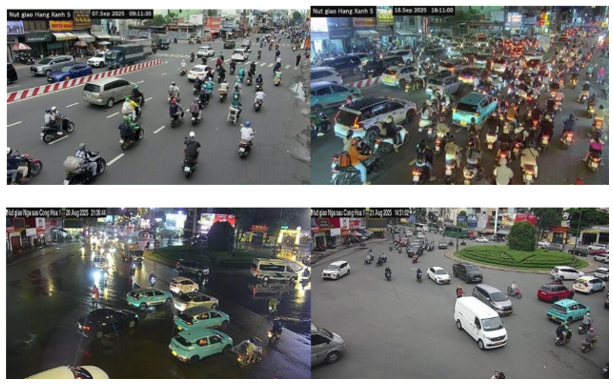
\includegraphics[width=\columnwidth]{fig/samples_pictures_get_from_api.png}
\caption{Sample surveillance camera feeds captured from the Ho Chi Minh City Traffic Portal API across diverse urban intersections.}
\label{fig:api_samples}
\end{figure}

\subsubsection{Graph Edges and RBF Adjacency Matrix}
Graph edges $\mathcal{E}$ represent physical road connections between adjacent camera stations. Edge weights $W_{ij} \in [0, 1]$ are derived from topological road travel distances $d_{ij}$ using a Radial Basis Function (RBF) kernel:
\begin{equation}
W_{ij} = \begin{cases} \exp\left(-\frac{d_{ij}^2}{\sigma^2}\right), & \text{if } i \neq j \text{ and } d_{ij} \le \tau \\ 0, & \text{otherwise,} \end{cases}
\end{equation}
where $\sigma$ is the standard deviation of road distances and $\tau$ is the spatial distance cutoff threshold.

The normalized Graph Laplacian $L$ and Scaled Laplacian $\tilde{L}$ are computed as:
\begin{equation}
L = I_N - D^{-1/2} W D^{-1/2}, \quad \tilde{L} = \frac{2}{\lambda_{\max}} L - I_N,
\end{equation}
where $D_{ii} = \sum_{j} W_{ij}$ is the diagonal degree matrix and $\lambda_{\max}$ is the maximum eigenvalue of $L$.

\subsubsection{Historical Feature Tensor and Target Horizon}
Outputs from Sub-problem 1 are aggregated at 5-minute intervals. Each node $i$ contains a 4-dimensional feature vector $\mathbf{x}_{i,t} \in \mathbb{R}^4$:
\begin{enumerate}
    \item Normalized total vehicle volume $v_{i,t}$.
    \item Sine time-of-day feature: $\sin\left(\frac{2\pi \cdot \text{tod}}{1440}\right)$.
    \item Cosine time-of-day feature: $\cos\left(\frac{2\pi \cdot \text{tod}}{1440}\right)$.
    \item Normalized hour of day: $\frac{\text{hour}}{24}$.
\end{enumerate}

Given historical time series over $T_{\text{in}} = 24$ steps (120 minutes of history), the historical input tensor is $X \in \mathbb{R}^{B \times T_{\text{in}} \times N \times F}$ ($F=4$). The target is forecasting future traffic volume across horizon $H = 6$ steps (30 minutes ahead): $Y \in \mathbb{R}^{B \times H \times N \times 1}$.

\subsection{Sub-Problem 2: TA-STGCN Network Architecture}

TA-STGCN couples Chebyshev Spectral Graph Convolutions \cite{chebnet}, 1D Gated Temporal Convolutions (GLU) \cite{stgcn}, and Model-Level Multi-Head Temporal Self-Attention \cite{attention}. Figure~\ref{fig:stgcn_architecture} illustrates the structural diagram of the TA-STGCN architecture.

\begin{figure}[htbp]
\centering
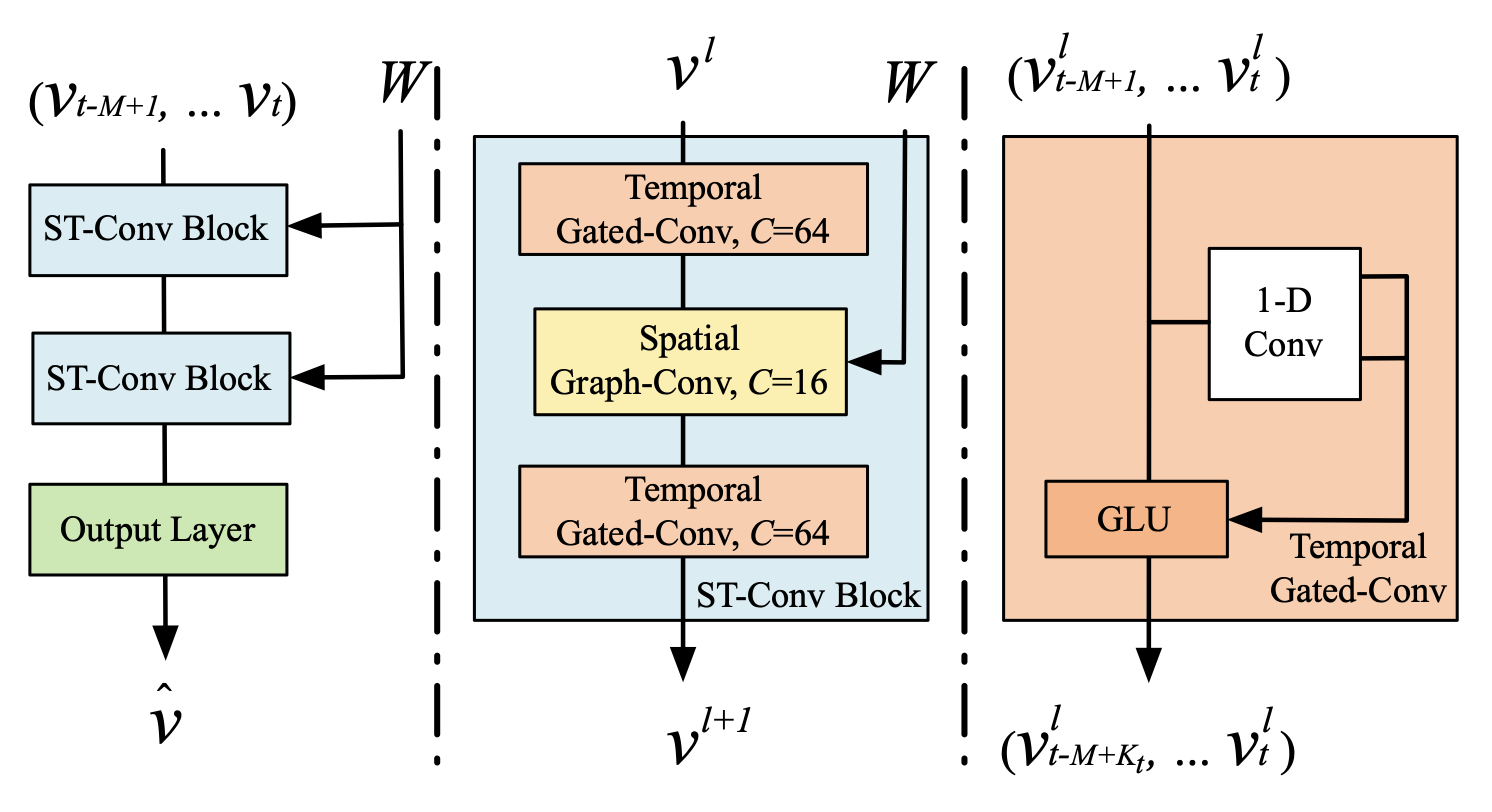
\includegraphics[width=\columnwidth]{fig/stgcn_architecture.png}
\caption{Architectural overview of TA-STGCN, integrating Chebyshev Spectral Graph Convolutions, 1D Temporal GLU blocks, and Model-Level Multi-Head Temporal Self-Attention.}
\label{fig:stgcn_architecture}
\end{figure}

\subsubsection{1D Temporal Gated Convolution (GLU)}
For feature map $H \in \mathbb{R}^{B \times C_{\text{in}} \times N \times T}$, 1D causal convolution doubles channels to $2 C_{\text{out}}$ \cite{stgcn}:
\begin{equation}
\text{Conv}_{1D}(H) = [P, Q] \in \mathbb{R}^{B \times 2 C_{\text{out}} \times N \times T'},
\end{equation}
\begin{equation}
\text{GLU}(H) = P \odot \sigma(Q) \in \mathbb{R}^{B \times C_{\text{out}} \times N \times T'},
\end{equation}
where $\odot$ denotes element-wise product and $\sigma(\cdot)$ is the sigmoid gate.

\subsubsection{Chebyshev Spectral Graph Convolution (ChebNet)}
Spatial graph convolution is approximated using truncated Chebyshev polynomials up to order $K=3$ \cite{chebnet}:
\begin{equation}
g_{\theta} \star_{\mathcal{G}} x \approx \sum_{k=0}^{K-1} \mathbf{\Theta}_k T_k(\tilde{L}) x,
\end{equation}
where $T_0(\tilde{L}) = I_N$, $T_1(\tilde{L}) = \tilde{L}$, and $T_k(\tilde{L}) = 2 \tilde{L} T_{k-1}(\tilde{L}) - T_{k-2}(\tilde{L})$.

\subsubsection{ST-Conv Block Assembly}
Each $ST\text{-Conv}$ block sandwiches spatial ChebNet graph convolution between two temporal GLUs with residual connection and LayerNorm \cite{stgcn}:
\begin{equation}
H^{(1)} = \text{GLU}_1(X), \quad H^{(2)} = \text{ReLU}\left( \text{ChebConv}\left(H^{(1)}, \tilde{L}\right) \right),
\end{equation}
\begin{equation}
H^{(3)} = \text{GLU}_2\left(H^{(2)}\right),
\end{equation}
\begin{equation}
H_{\text{block}} = \text{Dropout}\left( \text{LayerNorm}\left( H^{(3)} + \text{Residual}(X) \right) \right).
\end{equation}

\subsubsection{Model-Level Multi-Head Temporal Self-Attention}
To capture dynamic long-range temporal dependencies across the 24-step historical window, TA-STGCN applies \textbf{Multi-Head Temporal Self-Attention} \cite{attention} at the model output stage (post ST-Conv blocks).

The feature tensor $H_{\text{stgcn}} \in \mathbb{R}^{B \times C \times N \times T}$ is permuted and reshaped into node sequence batches:
\begin{equation}
Z = \text{Reshape}\left(\text{Permute}(H_{\text{stgcn}})\right) \in \mathbb{R}^{(B \cdot N) \times T \times C}.
\end{equation}

For $h=4$ attention heads \cite{attention}, Query, Key, and Value matrices are projected:
\begin{equation}
Q_m = Z W_m^Q, \quad K_m = Z W_m^K, \quad V_m = Z W_m^V, \quad m \in \{1, \dots, h\}.
\end{equation}
Scaled dot-product attention per head is computed as:
\begin{equation}
\text{head}_m = \text{Softmax}\left( \frac{Q_m K_m^T}{\sqrt{d_k}} \right) V_m, \quad d_k = C / h.
\end{equation}
\begin{equation}
\text{MHA}(Z) = \text{Concat}(\text{head}_1, \dots, \text{head}_h) W^O.
\end{equation}

A Transformer-style block \cite{attention} with residual connection, LayerNorm, and GELU Feed-Forward Network (FFN) updates temporal representations:
\begin{equation}
Z^{(1)} = \text{LayerNorm}\left( Z + \text{MHA}(Z) \right),
\end{equation}
\begin{equation}
Z^{(2)} = \text{LayerNorm}\left( Z^{(1)} + \text{FFN}(Z^{(1)}) \right),
\end{equation}
where $\text{FFN}(u) = \text{Linear}_{2}\left( \text{Dropout}\left( \text{GELU}\left( \text{Linear}_{1}(u) \right) \right) \right)$ with 4x dimension expansion ($C \to 4C \to C$).

\subsubsection{Output Conv1D Time-Reduction \& Objective Function}
The attention output tensor $Z^{(2)}$ is permuted back to $\mathbb{R}^{(B \cdot N) \times C \times T}$ and passed to a 1D output convolution with kernel size $T_{\text{in}}$ to collapse time dimension $T_{\text{in}} \to 1$:
\begin{equation}
\hat{Y} = \text{Reshape}\left( \text{Conv1D}_{T_{\text{in}} \to 1}\left(Z^{(2)}\right) \right) \in \mathbb{R}^{B \times H \times N \times 1}.
\end{equation}

The network is trained end-to-end using Pure Huber Loss \cite{huber} ($\delta = 1.0$):
\begin{equation}
\mathcal{L}_{\text{GNN}}(Y, \hat{Y}) = \begin{cases} \frac{1}{2}(Y - \hat{Y})^2, & \text{if } |Y - \hat{Y}| \le \delta \\ \delta |Y - \hat{Y}| - \frac{1}{2}\delta^2, & \text{otherwise.} \end{cases}
\end{equation}
